% Лекции Сергея Борисовича Стечкина
% ??? Внесены исправления В.И.Бердышева
% Внесены исправления Н.И.Черныха, версия 23.07.2009
% Внесена грамматическая и ТеХ-правка М.Дейкаловой, версия 05.08.09

 %%%%%%%%%%%%%%%%%%%%%%%%%%%%%
  %%%Лекция 8.
 \chapter{Наилучшие приближения в линейных нормированных пространствах}

 \section{Вспомогательные сведения из теории линейных \\ нормированных
 пространств}

{\it Линейное нормированное пространство} $X=(L,\|\cdot\|)$ -- это
 линейное пространство $L$ над полем вещественных или комплексных чисел,
 в котором введена норма -- функционал $\|\cdot\|:\ L\to [0,\infty),$
 удовлетворяющий аксиомам нормы:

1) $\|\lambda x\|=|\lambda|\cdot\|x\|,\ \lambda\in \mathbb R,\ x\in L;$

2) $\|x\|=0 \Rightarrow x=\theta,$
\ $\theta=\theta_X=0$ -- нуль пространства $X$;

3) $\|x+y\|\le \|x\|+\|y\|,\quad x,y\in L.$

 Если найдется ненулевой элемент $x,$ для которого $\|x\|=0$ и выполняются
 остальные аксиомы нормы, то $\|\cdot\|$ называется полунормой.

 Пусть дана произвольная линейная структура $L.$
 Имеют место следующие линейные (алгебраические) понятия.

\vspace{5mm}
{\bf 1.~Линейная зависимость и независимость}
\vspace{5mm}

Важную роль в $n$-мерном
 пространстве над полем $\bK$ (обычно $\bR$ или $\bC$) играет понятие линейной независимости.

 Конечная система элементов $x_1,\ldots,x_n$ из $L$ {\it линейно
 зависима}, если
 $$
 \exists\ {\{c_k\}_{k=1}^n \subset} \bK,\qquad {\sum\limits_{k=1}^n}|c_k|^2>0:\qquad \sum\limits_{k=1}^n
 c_kx_k=\theta.
 $$
 В противном случае система {\it линейно независима}.

 Размерность {пространства $L$} -- максимальное число {его} линейно независимых
 элементов, если оно конечно, и размерность пространства
 равна бесконечности, если для любого натурального $n$
 существуют линейно независимые системы $M \subset L$, {$M^{\#}=n$}
 {(т.\,е. мощность $M$ равна $n$)}

 Говорят, что {\it элементы бесконечного множества $M$ линейно независимы},
 если для любого натурального $n,$ не превосходящего мощность этого множества,
 и для любых различных $n$ элементов
 $x_1,\ldots,x_n$ из $M$ эти $n$ элементов линейно независимы.

 Говорят, что множество состоит  из линейно независимых элементов,
 если каждое его непустое конечное подмножество линейно независимо.

%\vspace{3mm}
 {\bf 2.~Алгебраический базис}
\vspace{5mm}

 Пусть $L_1 \subset L,$~ $L_1$ -- линейная подсистема. Говорят, что
 множество $M$ из $L_1$ есть {\it алгебраический базис} в $L_1,$ {если оно состоит из линейно независимых элементов и}
 если для любого $x\in L_1,$ $\ x\ne 0,$ существует такое $n$
 и существуют {различные элементы} $x_1,\ldots,x_n\in M$ такие, что
 $x=\sum\limits_{k=1}^n c_k x_k$, где
 не все $c_k=0$. {Из этого определения} {следует, что} если существуют еще и
 $y_1,\ldots,y_{{m}}\in M$ такие,
 что $x=\sum\limits_{k=1}^{{m}} d_k y_k,$ то {множества всех
 $\{x_k\}$ и $\{y_k\}$,} для которых
 $c_k\ne 0,$ {$d_l\ne 0,$} получаются друг из друга перестановкой,
 {при этом коэффициенты при равных элементах будут совпадать.}

 Во всякой линейной системе $L$ существует алгебраический базис $M$
 всего пространства.

 Действительно, вполне упорядочим элементы $L$
 $$
 x_1,\ldots,x_n,\ldots,x_{\omega_j},\ldots\,.
 $$
 {Будем говорить, что $x$ выражается через подмножество $A\subset L$, если $x$ есть линейная}
 {комбинация конечного числа элементов из $A$.}
 Вычеркнем $x_1$ и все элементы, которые через него выражаются;
 если оставшееся множество не пусто, первый его элемент
 обозначим через $\widetilde{x_2}$ и вычеркнем все
 элементы, которые линейно выражаются через $x_1, \widetilde{x_2}$
 и так далее, продолжая процесс по индукции (в общем случае трансфинитной, если $L$ не
 конечномерная система).
 Построенная система
 $x_1,\widetilde{x_2},\widetilde{x_3},\ldots$ -- конечная,
 счетная или трансфинитная будет, очевидно, алгебраическим
 базисом линейной системы $L.$

 Таким образом, в каждой линейной структуре
 существует алгебраический базис, и каждый элемент из $L$
 единственным образом, с точностью до нулевых
 коэффициентов, выражается через конечное число элементов базиса.

\vspace{5mm}
{\bf 3. Базис в линейных нормированных пространствах}
\vspace{5mm}

Пусть теперь
$X=(L,\|\cdot\|)$ -- линейное нормированное пространство.
Алгебраический базис существует в любом линейном
пространстве, в линейно нормированном же пространстве мы
будем рассматривать другой вид базиса.

 Множество $M$ называется базисом в линейном нормированном
 пространстве $X,$ если любой $x\in X$ единственным образом,
 с точностью до нулевых коэффициентов, представляется в виде
 $$
 x=\sum\limits_{k=1}^{\infty} c_kx_k,
 $$
 где $x_k\in M,$~ $c_k\ne 0;$ {и равенство означает, что} ряд сходится в
 смысле нормы пространства {и его сумма совпадает с $x$.}

 Базис здесь не обязан быть счетным, но для любого $x$
 найдется не более чем счетное множество элементов $x_k\in M$
 такое, что $x=\sum\limits_{k=1}^{\infty}c_kx_k.$

 Известно, что если пространство сепарабельно
 (т.\,е. имеет счетное всюду плотное множество) и не является конечномерным,
 то всякий его базис счетный. В этом случае $x=\sum\limits_{k=1}^{\infty} c_kx_k,$
 т.\,е. $x$ выражается рядом из всех элементов базиса и некоторые $c_k$
 могут равняться нулю. При этом, если сумма ряда (предел последовательности частичных сумм
 $\sum\limits_{k=1}^{n} c_kx_k$) не зависит от перестановки членов
 ряда, то базис $x_1,x_2,\ldots$ называется безусловным.
 Если последнее свойство не гарантировано, то базис
 называется базисом Шаудера.

 \task %%% Задача.
 Всякое ли сепарабельное банахово пространство имеет
 базис?\footnote{П.\,Энфло построил (1972 г.) отрицательный пример.}

 Доказано (З.\,Чесельский), что во всех классических
 сепарабельных банаховых пространствах существует базис,
 т.\,е., например, в пространствах $C,$~ $L^p\ (p>1),$~ $C^{(r)},$~ $C^{\infty}.$

 \vspace{5mm}
 {\bf 4.~Выпуклость}
 \vspace{5mm}

   Множество $M\subset L$ называется {\it выпуклым},
 если для любых пар точек $x,y\in M$ отрезок $[x,y]\subset M.$
 Отрезок $[x,y],$ соединяющий пару точек $x,y,$ есть множество
 точек пространства вида
 $$
 tx+(1-t)y,\qquad t\in [0,1].
 $$

 Множество $M$ будет {\it невыпуклым}, если найдутся две такие точки
 множества, что на соединяющем их отрезке не все точки принадлежат
 множеству (рис.~8.1).
 \vspace{7mm}

  \begin{figure}[ht]
\begin{center}

\includegraphics[width=0.6\textwidth]{pict08-1.eps}
\end{center}
 \bigskip
 \refstepcounter{ris}\label{r8-1}

 \centerline{Рис.~\theris}
 \bigskip
\end{figure}

%\vspace{5mm}


  {Классы выпуклых множеств в конечномерных и бесконечномерных} пространствах
 сильно различаются. Например, в
 любом бесконечномерном банаховом пространстве существуют два выпуклых
 множества таких, что каждое из них всюду плотно в пространстве,
 объединение их есть все пространство и они не пересекаются.

\vspace{5mm}
{\bf 5.~Выпуклая оболочка} {(это алгебраическое понятие)}
\vspace{5mm}

Пусть $L$ -- линейное пространство и
 $M\subset L.$ Рассмотрим всевозможные выпуклые множества
 $V\supset M,$~ $V\subset L.$

 {\it Выпуклой оболочкой} $\conv M$ называется множество
 $$
 \conv M=\bigcap_{V\supset M} V.
 $$
 Ясно, что $M\subset \conv M.$ Выпуклая оболочка
 всегда существует, так как $V=L\supset M.$

 \ex
 Доказать, что множество $M$ выпукло тогда и только тогда, когда $M$
 совпадает со своей выпуклой оболочкой.

{Обсудим}, как в общем случае устроена выпуклая оболочка $\conv M$.

 Возьмем любое конечное подмножество $M_n=\{ x_1,\ldots,x_n\}\subset M.$
 Составим его выпуклую оболочку (симплекс размерности $n-1,$
 если $x_1,\ldots,x_n$ -- линейно независимые элементы) -- $\conv M_n$ (рис.~8.2).

 %\vspace{2cm}
 %%%%%%%%%%%%%%%%%%%%%%%%%%%%%%%%%%%%%%%%%%%%%%%%%%%%%%
 %\hbox to 0.5cm {}{\special{em:graph pict1.pcx}}
 %\vspace{6cm}
 %%%%%%%%%%%%%%%%%%%%%%%%%%%%%%%%%%%%%%%%%%%%%%%%%%%%%%%%%%
\vspace{10mm}


  \begin{figure}[ht]
\begin{center}
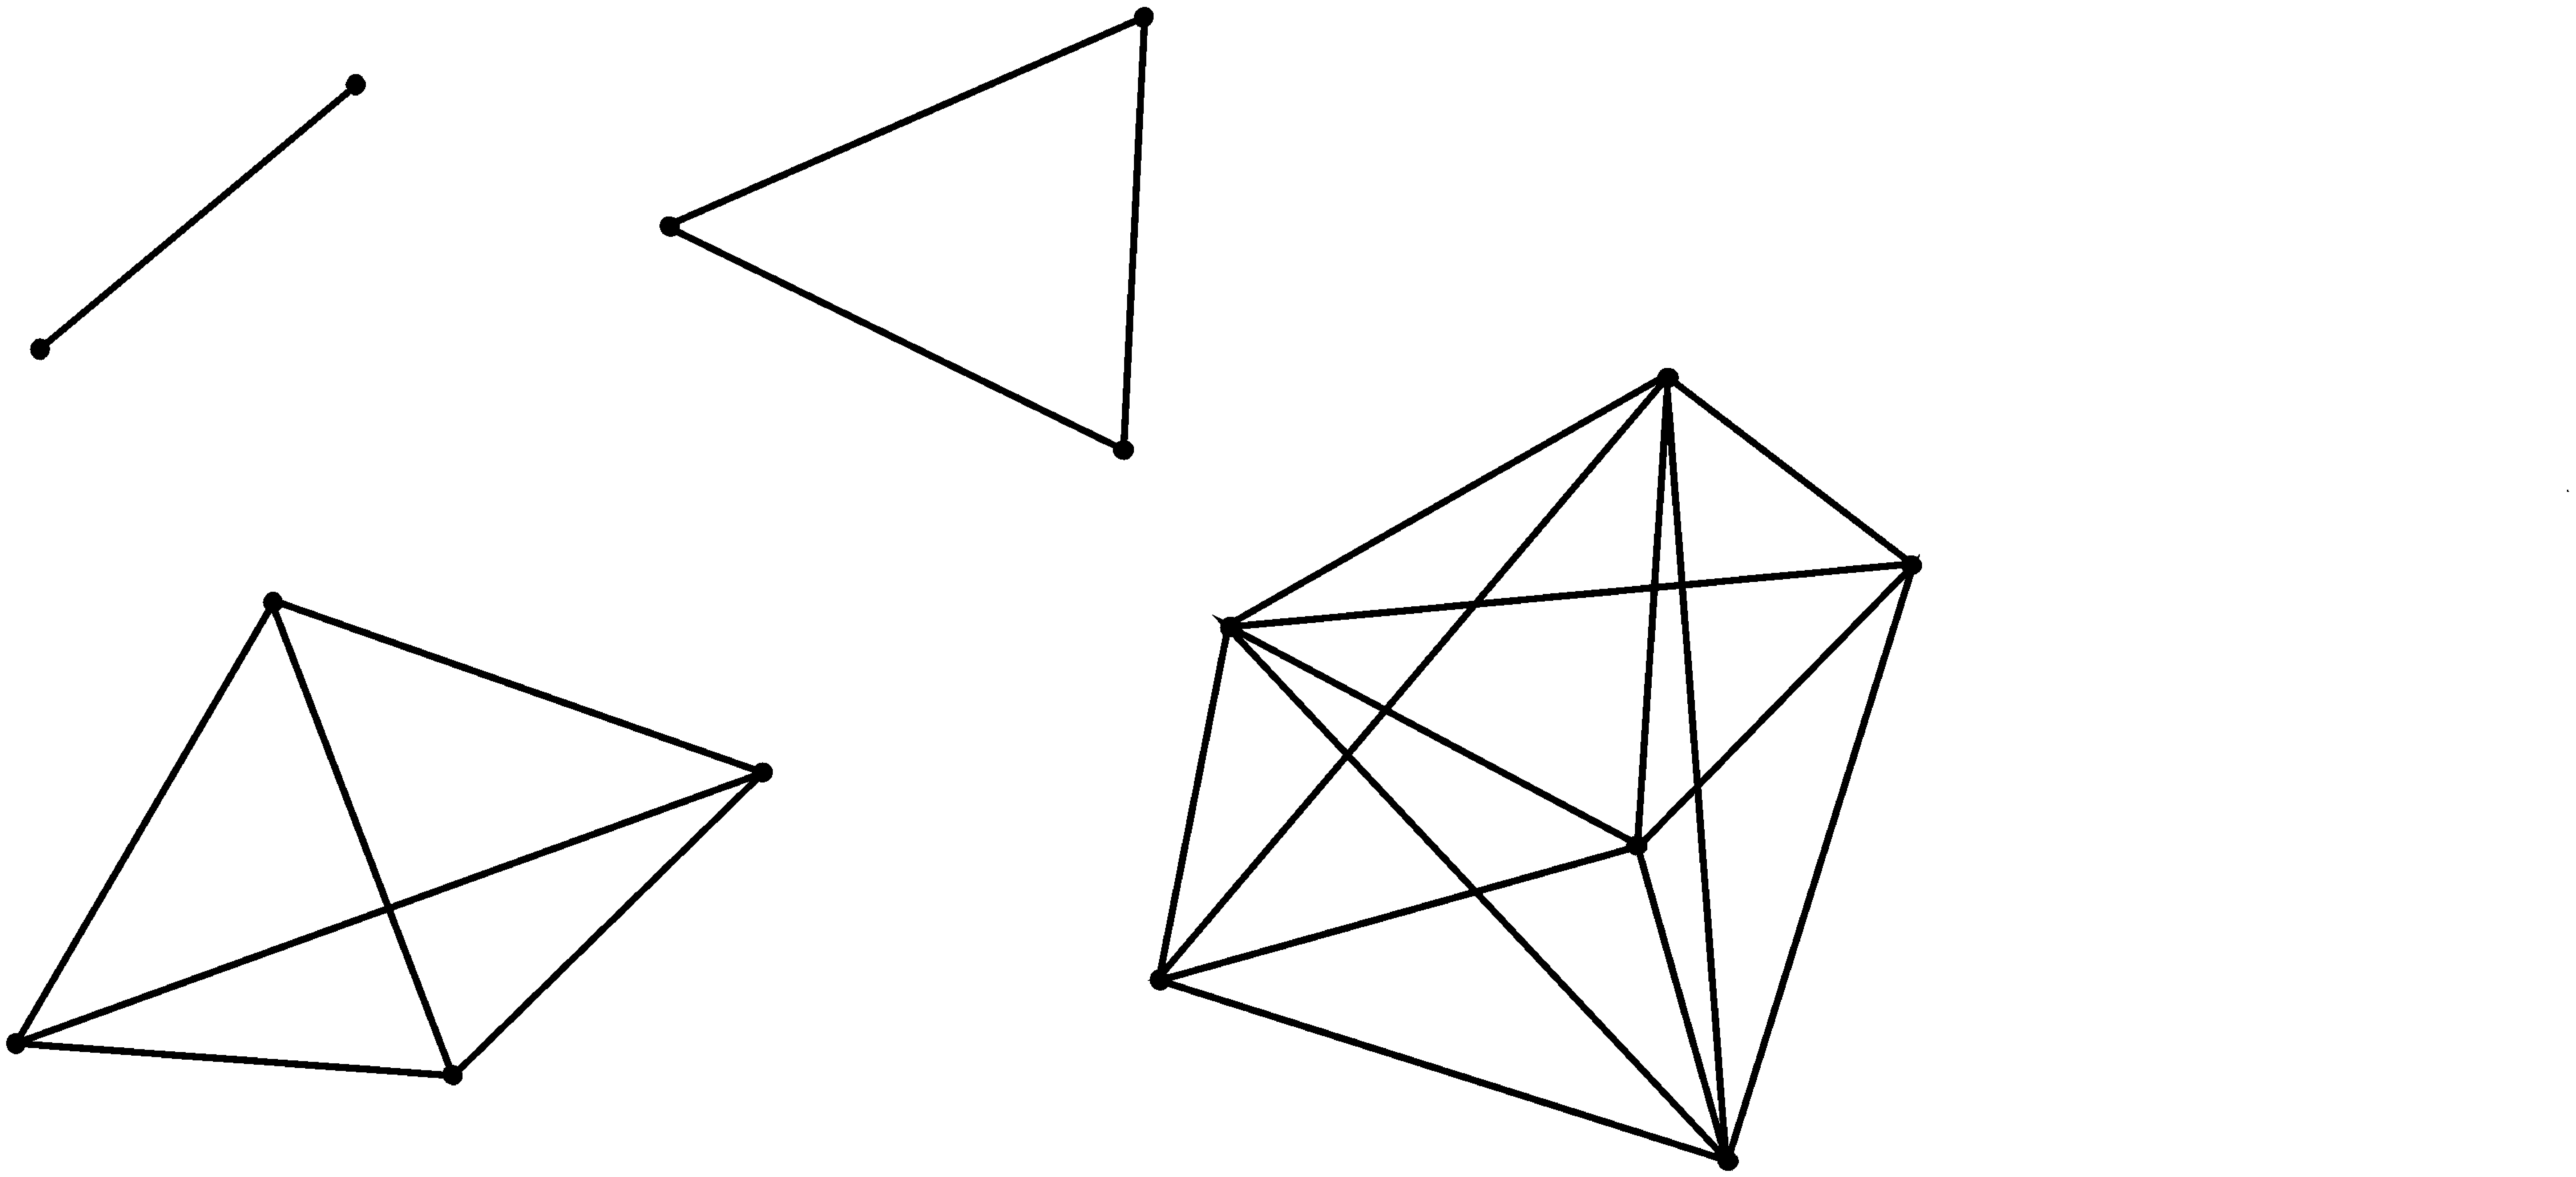
\includegraphics[width=0.6\textwidth]{pict08-2.eps}
\end{center}
 \bigskip
 \refstepcounter{ris}\label{r8-2}

 \centerline{Рис.~\theris}
 \bigskip
\end{figure}

 \vspace{5mm}

Оказывается,
 $$
 \bigcup_{M_n\subset M} \conv M_n=\conv M.
 $$
 Действительно, пусть $x,y$ принадлежат
 $ \bigcup\limits_{M_n\subset M} \conv M_n,$
 тогда $x$ принадлежит некоторому симплексу $\conv M_n,$
 а $y$ принадлежит некоторому симплексу $\conv M_m.$
 Следовательно, $x$ и $y$ принадлежат {симплексу} $\conv M',$ где $M'=M_n
 \bigcup M_m$ и $[x,y]\subset \conv M' \subset
 \bigcup\limits_{M_n\subset M} \conv M_n.$ Таким образом, $\bigcup
 \conv M_n$ выпукло. {Ясно, что это множество} принадлежит любому выпуклому множеству $V,$
 содержащему $M,$ и есть их пересечение.

 \begin{Corollary} %%% Следствие.
 {Множество}
 $$
 \bigcup_{M_n\subset M} \conv M_n
 $$
 есть наименьшее выпуклое множество, содержащее $M.$
 \end{Corollary}

 \begin{Remark} %%% Замечание.
 Если $x_1,\ldots, x_n\subset M,$ то $\conv M_n$ {совпадает с множеством}
 $$
 \left\{x=\sum\limits_{k=1}^n c_kx_k:\quad c_k\ge 0,\quad \sum\limits_{k=1}^n
 c_k=1\right\}.
 $$
 \end{Remark}

Бывает нужна также {\it замкнутая выпуклая оболочка} $\overline{\conv M}$
множества $M.$

\ \

\section{Характеристики линейных нормированных пространств}

{\bf 1.~Сепарабельность}
\vspace{3mm}

Характеристикой массивности пространства является
 наименьшая мощность всюду плотного множества.

 Пространство, для которого существует всюду
 плотное счетное множество, называется {\it сепарабельным}.

 Пространство, не совпадающее с $\theta$ и в котором нет всюду
 плотного счетного множества, называется {\it несепарабельным}.

 Первое, что мы должны проверять для пространства -- сепарабельность.

\vspace{5mm}
{\bf 2.~Полнота}
\vspace{5mm}

Пространство называется {\it полным}, если всякая последовательность
 Коши (фундаментальная последовательность) является сходящейся к
 какому-либо элементу пространства.

 Полное линейное нормированное пространство
 называется {\it банаховым пространством} или пространством
 типа $B.$

\vspace{5mm}
{\bf 3.~Рефлексивность}
\vspace{5mm}

Пусть $X$ -- банахово пространство; $X^*$ -- сопряженное с ним
 пространство линейных непрерывных функционалов, всегда банахово; $X^{**}$ -- второе
 сопряженное пространство.

 Существует каноническое вложение $X$ в $X^{**}$ посредством формулы:
 {для любого} {$x\in X$ положим}
 $$
 F_{{x}}(f)=f(x),\qquad f\in X^*,
 $$
 так что
 $$
 \forall\ x\in X\qquad x\longmapsto F_{{x}}\in X^{**}.
 $$

 Пространство называется {\it рефлексивным}, если при
 каноническом вложении $X$ в $X^{**}$ на самом деле имеем $X\equiv X^{**}$,
 {т.\,е. любой функционал}
 {$F\in X^{**}$ совпадает с некоторым функционалом}
 {$F_x$ над $X^*$.}

 Если пространство рефлексивно, то $X$ и $X^{**}$ устроены одинаково (изоморфны и изометричны).
 Обратно неверно, $X$ и $X^{**}$ могут быть, например, изоморфны, но
 $X$ не рефлексивно.

 Известно, что если  пространство рефлексивно,
 то из любой ограниченной последовательности
 его элементов можно выбрать слабо сходящуюся подпоследовательность.

\vspace{5mm}
 {\bf 4.~Строение сферы (шара)}
 \vspace{5mm}

 {\bf \normalsize   a) Строгая выпуклость.} Пространство называется {\it строго выпуклым},
 если его единичный шар строго выпуклый.

 Единичный шар строго выпуклый, если для любых $x\ne y,$ принадлежащих шару, любая точка
 на интервале $(x,y)$
 лежит строго внутри шара.

 \begin{Example} %%% Пример.
 Круг -- строго выпуклое множество (рис.~8.3), квадрат -- не строго
 выпуклое. Ясно, что если пространство не строго выпуклое,
 то существует гиперплоскость, которая касается единичного
 шара более, чем в одной точке.

 \vspace{0.5cm}
 %%%%%%%%%%%%%%%%%%%%%%%%%%%%%%%%%%%%%%%%%%%%%%%%%%%%%%
 %\hbox to 0.5cm {}{\special{em:graph pict1.pcx}}
 %\vspace{6cm}
 %%%%%%%%%%%%%%%%%%%%%%%%%%%%%%%%%%%%%%%%%%%%%%%%%%%%%%%%%%
 \begin{figure}[ht]
\begin{center}
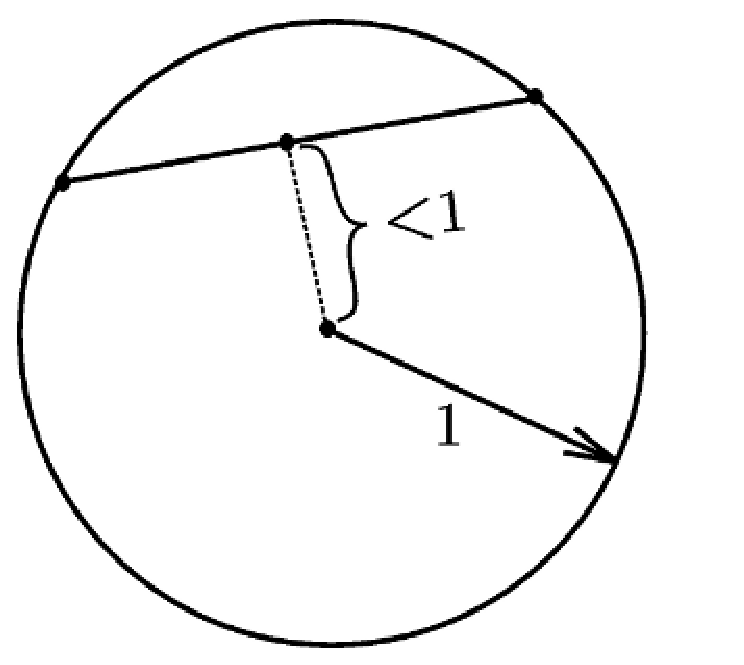
\includegraphics[width=0.3\textwidth]{pict08-3.eps}
\end{center}
 \bigskip
 \refstepcounter{ris}\label{r8-3}

 \centerline{Рис.~\theris}
 \bigskip
\end{figure}
 \end{Example}

 {\bf \normalsize b) Экстремальные точки} {(это линейное понятие).}
 Пусть множество $M\subset X,~ x\in M.$

 Точка $x\in M$ называется {\it неэкстремальной} точкой множества $M,$
 если существуют точки $a,b\in M$ такие, что $x\in (a,b)$
 (рис.~8.4). В противном случае точка называется {\it экстремальной}.

%\newpage

 %\vspace{2cm}
 %%%%%%%%%%%%%%%%%%%%%%%%%%%%%%%%%%%%%%%%%%%%%%%%%%%%%%
 %\hbox to 0.5cm {}{\special{em:graph pict1.pcx}}
 %\vspace{6cm}
 %%%%%%%%%%%%%%%%%%%%%%%%%%%%%%%%%%%%%%%%%%%%%%%%%%%%%%%%%%
   \vspace{10mm}
\begin{figure}[ht]
\begin{center}
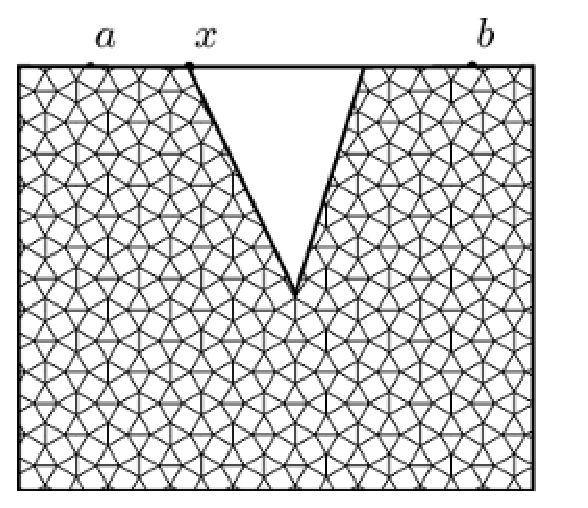
\includegraphics[width=0.3\textwidth]{pict08-4.eps}
\end{center}
 \bigskip
 \refstepcounter{ris}\label{r8-4}

 \centerline{Рис.~\theris}
 \bigskip
\end{figure}

\vspace{5mm}



 Пусть $O_1$ -- единичный шар, $S_1$ -- сфера, его граница.

 {Имеет место}
 \begin{teo}
 В любом конечномерном банаховом пространстве шар $O_1$ есть
 замкнутая выпуклая оболочка своих экстремальных точек.
 \end{teo}

 Теорему приводим без доказательства. В общем случае она неверна. Существуют банаховы
 пространства, в которых единичный шар не имеет
 экстремальных точек.

 \ex
 Доказать, что в единичном шаре $O_1$  в $L{[0,1]}$ нет ни
 одной  экстремальной точки.

 \ex
 Доказать, что шар $O_1$ в $C[0,1]$ имеет две экстремальных точки.

\vspace{5mm}
 {\bf \normalsize c) Гладкость.}
 Пространство называется {\it гладким}, если для любой
 точки на $S_1$ существует единственный опорный функционал,
 т.\,е. единственная касательная гиперплоскости.
 Определение касательной гиперплоскости будет дано позже.

 В противном случае пространство не гладко.

\vspace{5mm}
 {\bf 5.~Компактные множества}
 \vspace{5mm}

  Компактное множество -- такое множество, из любой
 последовательности
 которого можно выбрать сходящуюся подпоследовательность к элементу этого множества.

 Компактное множество всегда замкнуто.

 \vspace{3mm}
 \section{Основные пространства}
  \vspace{3mm}

 {\it Пространство $C=C(Q,X)$ -- это пространство непрерывных функций}, определенных
 на компакте $Q$ и принимающих значения из банахова пространства $X.$
 Классические случаи: $X=\bR,$  $\ X=\bC.$
 \vspace{3mm}

 1. {Пространство $C(Q,X)$} полное.
 \vspace{3mm}

 2. При некоторых $Q$ и $X$ пространство {$C(Q,X)$} сепарабельно, а при некоторых -- нет.

 Если $Q$ -- отрезок, $X=\bR,$ то $C(Q,X)$ сепарабельно.
  \vspace{3mm}

 3. Если $Q$ бесконечно, то $C$ нерефлексивно; в частности, $C[0,1]$ нерефлексивно.
  \vspace{3mm}

 4. {При любых $Q,$ $X$ пространство $C(Q,X)$} не строго выпуклое пространство {и не} {гладкое.}
\vspace{3mm}

 \ex %%%Упражнение.
{Доказать эти свойства.}

{{\it Пространство} $ L^{{p}},~ 1\le p< \infty.$}

 Пусть задано пространство $Q$ с мерой $\mu$ ($\mu$ --
 счетно аддитивная неотрицательная функция измеримых подмножеств из $Q$).

 Пусть $y=f(x)$ -- определенная на $Q$ измеримая
 функция {со значениями в $\bR$ или $\bC$,} для которой
 интеграл  $\ds\int_Q |f(x)|\ d\mu$ конечен, $L_{{\mu}}$ -- множество таких функций и
 $\ds\int_Q |f(x)|\ d\mu=\pnl f\pnr$ -- полунорма.
 Для того, чтобы получить банахово пространство, факторизуем $L_{{\mu}}$:
 $$
  \left. L_{{\mu}} \right/ \{f:\ \pnl f\pnr =0{\}},
  $$
 {т.\,е. будем отождествлять функции, различающиеся лишь на подмножестве нулевой} {меры.}
 Получим полное пространство, которое и далее будем обозначать $L_{{\mu}}.$

 Сепарабельность $L_{{\mu}}$ зависит от $Q$ и от $\mu;$ если $\mu$ --
 мера Лебега на $Q\subset\bR^n,$ то $L_{\mu}=L_{\mu}^1(Q)=L(Q)$ сепарабельно.

 Чтобы получить $L^p_\mu$, возьмем полунорму
 $$
 \pnl f \pnr =\left( \int_Q |f(x)|^p\, d\mu \right)^{1/p}.
 $$
{ Класс эквивалентности, соответствующий функции $f$, будем обозначать тем же}
{символом $f$ и потому $\pnr f\pnr=\|f\|_{L^p}$ -- норма.}

 При $p=2$ получим {$L^2_\mu$} -- гильбертово пространство со скалярным
 произведением
 $$
 (f,g)=\ds\int_Q {fg}\ d\mu
 $$
 над полем действительных чисел,
 $$
 (f,g)=\ds\int_Q {f{\overline g}}\ d\mu
 $$
 над полем комплексных чисел; {$L^2_\mu$}~--
 полное относительно нормы $\|f\|_{{L^2}}=\sqrt{(f,f)}$ {пространство}.

 Напомним, что в пространствах $L^p,\ L^q,$ при $\dfrac{1}{p}+\dfrac{1}{q}=1,\ 1<p,\ q<\infty$
 неравенство Г\"{е}льдера
 $$
 \left| \int_{a}^b f(x)g(x)\,dx\right| \le
 \|f\|_{L^p[a,b]}\|g\|_{L^q[a,b]}
 $$
 для $f\in L^p[a,b],\ g\in L^q[a,b]$ превращается в
 равенство только если $f(x)g(x)\ge 0$ почти всюду и
 $|f(x)|^p$ почти всюду пропорционален $|g(x)|^{q}.$

 \begin{ex}
Рассмотреть эту задачу для функций их $L^p_{\mu}(Q)$ и $L^q_{\mu}(Q).$
 \end{ex}
